\chapter{Mérések}

Ebben a fejezetben az elvégzett mérésekről lesz szó, illetve azokból levont konklúziókról. Megnézzük, hogy a dolgozatban elkészített szoftverrendszer milyen hatékonysággal működik, milyen feltételekkel és minek milyen hatása van a QoS paraméterek elmozdulására. Kitekintünk arra, hogy egy 5G-s közeghozzáférési technológia esetén milyen változás jelenne meg a kommunikációban, elgondolkodunk rajta, hogy ez milyen előnyöket jelenthet. A méréseket az elkészített virtuális Multipass alapú K3S rendszeren végeztem, a mérési architektúra a korábbi \ref{fig:full2drone}. ábrán látható. A méréseket úgy végeztem, ahogyan a kapcsolóállomásba is implementáltam a valós idejű méréseket, annyi különbséggel, hogy nagyobb adatot átlagoltam a pontosság érdekében. \\

\noindent
Két fontos dologra vagyunk kíváncsiak:
\begin{itemize}
	\item A kapcsolóközpont viselkedése, meghibásodott Node esetén
	\item A kapcsolóközpont viselkedése nagy késleltetés esetén
	\item A drónok számának növekedése esetén hogyan alakul a válaszidő és a sávszélesség
	\item Flotta irányítása esetén a válaszidő és a flotta méretének kapcsolata
\end{itemize}

\section{Node váltás ideje meghibásodott Node esetén}
A drónkapcsoló állomás hiba esetén átvált egy backup node-ra, ahol ugyanaz a munka folytatódik, amit a drón megkezdett. A kapcsolóállomásba implementált \emph{timestamp} alapú naplózórendszer segített abban, hogy pontos idők kapjak a reakcióról és a helyreállásról. A mérés menete egy drón normál üzemben működése közben:
\begin{enumerate}
	\item Hibát idézünk elő, kikapcsoljuk azt a Node-ot amelyen fut a Roscore és rögzítjük az időt (\ref{lst:close}. lista) ($t_0$)
	\item Megvárjuk amíg a kapcsolóállomás fel nem ismeri a hibát. ($t_1$)
	\item Megvárjuk amíg talál egy új Node-ot és helyreáll az üzem. ($t_2$)
\end{enumerate}

\begin{lstlisting}[caption={Node kikapcsolása}, label={lst:close}]
date +%s && multipass stop worker-1
\end{lstlisting}

\noindent
$t_2-t_1$ helyreállási időre minimálisan 0.8, maximálisan 2.18, átlagosan 1.15 másodpercet mértem 10 mintavételezésből. $t_1-t_0$ észrevételi időt több periódusidővel is kipróbáltam, mindegyikkel öt-öt mérést átlagolva.
\begin{itemize}
	\item $5s$ ellenőrzési periódusidő esetén: $2.3s$
	\item $10s$ ellenőrzési periódusidő esetén: $6.1s$
	\item $15s$ ellenőrzési periódusidő esetén: $8.5s$
\end{itemize}

\noindent
Ez azt jelenti, hogy a jelentős késleltetést az ellenőrzések periódusából adódó késleltetés adja, amelynek periódusa alatt egyenesen oszlik el a várható keletkező hiba. Így annak beállítását a felhasználó mérlegelheti, hogy mennyire kritikus a drón munkája és mennyire lehet terhelni a hálózatot. Észrevétel után a kapcsolási idő már csak pár másodperc. Ha például $5s$-os hibajavítást szeretnénk, akkor $5s$-ra kell állítani az ellenőrzési periódusidőt. Fontos megjegyezni, hogy ezen kiesési idő alatt a drónnak kell valamilyen belső mechanizmussal rendelkeznie, amely tovább viszi a feladatot vagy hagyja biztonságosan lebegni a következő utasításig, amennyiben nem érkezik válasz egy bizonyos időkereten belül. A piacon található középkategóriás drónok rendelkeznek ilyen viselkedéssel, ipari használatban pedig fontos, hogy ilyen kritériummal ruházzanak be drónra.

\section{Válaszidő különbség esetén a jobb Node kiválasztása}
A drónkapcsoló állomás nem csak akkor vált át másik Node-ra ha az aktuálisan felhasznált worker Node kiesik, hanem akkor is ha egy bizonyos $p$ paraméterrel alacsonyabb a válaszidő az adott Node felől, a legalacsonyabb elérhető válaszidőhöz képest. Ennek váltási algoritmusa részletesebben a \ref{cha:alg}. fejezetben részleteztem. A mérést hasonlóan végeztem, mint az előzőt, azonban mással implikáltam a változást, nem megszűntettem működés közben a Node-ot, hanem a Node belső interfészéhez hozzáadtam egy 0.5s-os késleltetést, hogy kívülről elérve a virtuális rendszerben ennyi késleltetés adódjon hozzá mindenféle kommunikációhoz (\ref{lst:tc}. lista). Ennek rögzítettem az idejét és vártam az algoritmus ellenőrző mechanizmusát és a Node váltás bekövetkeztét.

\begin{lstlisting}[caption={Késleltetés hozzáadása a worker Node külső interfészéhez alapértelmezett Linux programmal}, label={lst:tc}]
tc qdisc add dev ens4 root netem delay 500ms
\end{lstlisting}

\noindent
Az eredmény hasonló lett, tíz mintavételből a teljes interfész lassítás után minimum 3.2, maximum 6.91, átlagosan pedig 4.2 másodperc alatt történt meg a Node váltás, 5 másodperces ellenőrzési periódussal mérve.

\section{Terheltségi válaszidő viszonya}
Következőnek azt néztem meg, hogy a virtuális rendszerben hogyan terhelődik a klaszter az irányítandó drónok számának növekedvén. Egy drónhoz tartozik három konténer a klaszterben, abból a Roscore-ból kettő van, mindkét worker Node-on, így összesen négy konténer tartozik egy drónhoz. A méréseket egy kitüntetett drón és hozzá tartozó Roscore között végeztem, akkor is amikor több drón volt a rendszerben.\\

\begin{figure}
	\centering
	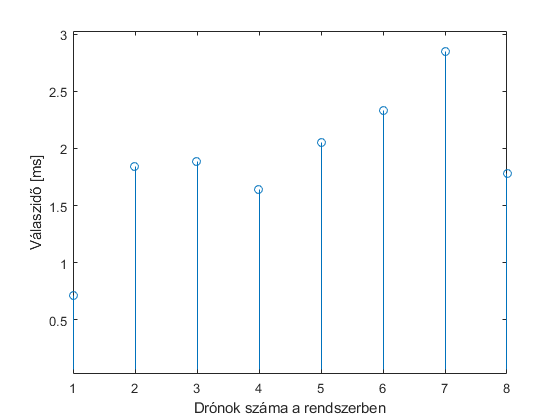
\includegraphics{figures/meres_ping.png}
	\caption{Válaszidő a drónok számának függvényében}
	\label{fig:meresping}
\end{figure}

\noindent
A válaszidőt 25 ICMP ping visszaérkezési idők átlagaként számoltam ki, úgy hogy a drón virtuális konténeréből küldtem a Roscore konténer interfészére. Az eredményen az látszik, hogy nő az üzemeltetett konténerek függvényében a válaszidő, nem drasztikusan, azonban valamilyen lineáris görbére illeszthetően (\ref{fig:meresping}. ábra).  \\

\begin{figure}
	\centering
	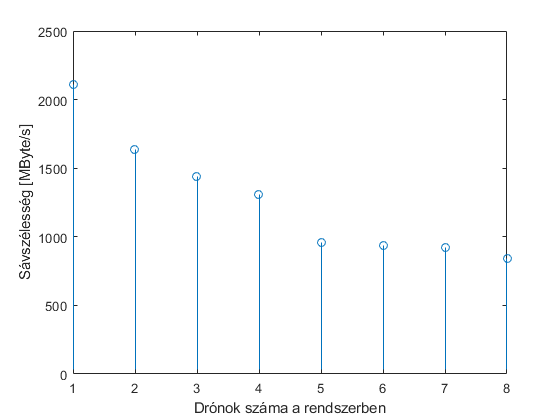
\includegraphics{figures/meres_iperf.png}
	\caption{Sávszélesség a drónok számának függvényében}
	\label{fig:meresiperf}
\end{figure}

\noindent
A sávszélességet \emph{iperf3} programmal néztem, szintén egy drón konténer és a hozzá tartozó Roscore között, melyből a következő eredményt kaptam (\ref{fig:meresiperf}. ábra). A sávszélesség csökkenése is észrevehető, ugyan nincs mögötte az a linearitás, mint a válaszidő növekedésében, egy drónhoz képest megfeleződött a rendelkezésre álló kiszolgáltatott sávszélesség a klaszter felől. Az \emph{iperf3} program a rendelkezésre álló szabad sávszélességet mutatja meg, melyet teljes terhelés alatt mér meg egy rövid időablakban. Alaphelyzetben, egyetlen drón kapcsolatba lépése nélkül a két konténer között $f_{0}=2430 MB/s$-ot mértem a hálózat terhelésével. Ez azt jelenti, hogy drón kommunikáció nélkül ennyivel terhelhető a hálózat a két konténer között, amelyet a hardver és a virtualizáció határoz meg. Ez $f_0$ kezdeti értékre és kiszámított $f$ függvény pontjaira illeszthető görbe a GeoAlgebra függvényillesztő segítségével \[ f(n) = e^{-0.47n} \cdot 1397.25 [MB/s]\] eredmény jött ki, ahol $n$ a rendszerben lévő drónok száma. \\

\begin{figure}
	\centering
	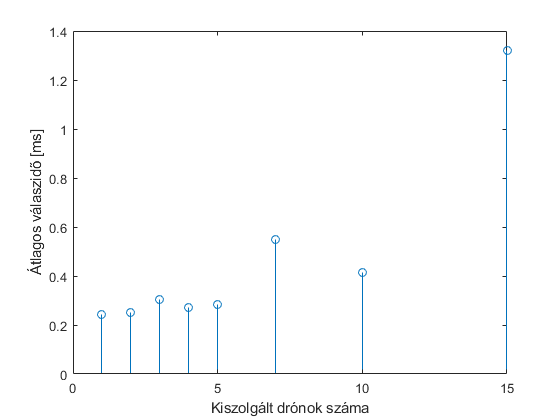
\includegraphics{figures/meres_ros.png}
	\caption{Kiszolgálási válaszidő a drónflotta méretének függvényében}
	\label{fig:meresros}
\end{figure}

\noindent
Az \ref{cha:toki} fejezetben vizsgáltuk a matematikai modelljét egy M/M/1 kiszolgálási Erlang rendszernek. A diplomatervezés folyamatában a ROS rendszernek a megismerése közben kiderült, hogy a jelenlegi irányító szoftver arra nincs felkészítve, hogy egy Roscore-on keresztül irányítson több drónt, illetve az általam megalkotott végső Kubernetes rendszerben minden drónnak külön Roscore-ja van. Azért megnézzük, hogy mi lenne akkor ha lenne egy ROS-on keresztül N résztvevőjű flottát irányító szoftverünk, amely egy Roscore-on keresztül vezérelné a flottát. A mérést egy drón konténere és az egyetlen Roscore között végeztem a felhőben. A tiszta mérés kedvéért nem deploy-oltam az irányításra és kamerafeldolgozásra szolgáló konténereket. Egy és tizenöt drón között mértem a válaszidőt a ping programmal, 25 visszapattanást átlagolva (\ref{fig:meresros}. ábra). Jól látszik, hogy növekszik a drónok növelésével az egy drón felé lehetséges kiszolgálási idő. Tehát növekszik az \ref{cha:toki}. fejezetben megmutatott $\mu$ érték, amely fordítottan arányos a késleltetéssel.

\section{Késleltetés hozadéka 5G közeghozzáférés esetén}
A mérésekben megnéztük, hogy milyen késleltetések és sávszélességek vannak egy teljesen virtualizált rendszerben. Egy valós hálózaton és fizikai drónnal működő rendszerrel még hozzájön két rendszerből származó érték ezekhez a késleltetésekhez és sávszélességekhez. Értelemszerűen a késleltetéshez hozzáadódik, a sávszélességnél pedig az értékek minimumára csökken. \\

\noindent
A hálózat késleltetése és a közeghozzáférési technológia késleltetése adódik hozzá a teljes válaszidőhöz. A tanszéken kipróbált Wifi-s közeghozzáférés körülbelül $300 ms$-ot növel a szimulációhoz képest. Az 5G $5-15 ms$ körüli értéket is biztosíthat, így ezzel a technológiával minimalizálni lehet a teljes késleltetést az előző pontban kiszámoltakhoz konvergálva.